%!TEX root = ../crux.tex

% THIS IS AN EXAMPLE DOCUMENT FOR VLDB 2012
% based on ACM SIGPROC-SP.TEX VERSION 2.7
% Modified by  Gerald Weber <gerald@cs.auckland.ac.nz>
% Removed the requirement to include *bbl file in here. (AhmetSacan, Sep2012)
% Fixed the equation on page 3 to prevent line overflow. (AhmetSacan, Sep2012)


\section{Introduction}
\label{sec:intro}

Structured data repositories, such as knowledge bases, taxono\-mies, and hierarchies, have recently been used to power end-user applications of many types, including keyword search engines, question answering systems, event detection and prediction algorithms, as well as recommender systems. For instance, a number of companies, including Google~\cite{singhal2012introducing}, Microsoft~\cite{cheng2010fuzzy}, Walmart~\cite{Deshpande:2013:BMU:2463676.2465297}, Yahoo~\cite{woo}, and Amazon~\cite{amazon-product}, all leverage structured data repositories for organizing and serving information for various applications. 

All these repositories critically rely on fully automated information extraction mechanisms that combine methods from pattern matching, computational linguistics, and statistical learning with precompiled dictionaries containing patterns of interest, synonyms, etc under a closed-world assumption. Often, these dictionaries tend to have limited coverage, and focus only on {\em head data}, i.e., data about popular entities, facts, and attributes, thus, most repositories leave behind a considerable volume of fine-grained data belonging to the {\em long tail}. To optimally benefit from using these repositories, it is essential that we augment them with long tail data, and keep that up-to-date. 

In the recent past, {\em crowdsourcing} has proven to be a natural alternative for overcoming the fundamental limits posed by following a closed-world assumption~\cite{franklin:2011}. In fact, it has been shown that crowdsourcing can leverage human intelligence to provide us access to fine-grained information~\cite{deco}. Also, initial studies~\cite{trushkowsky:2013, amsterdamer:2014} have shown that crowdsourcing provides a viable alternative for extracting entities by following a micro-task based approach that asks humans to ``list one more entity'' from a predetermined domain. For example, if we consider the task of enumerating all people mentioned in today's issue of New York Times, previous techniques focus on issuing the query ``list one person in today's New York Times'' repeatedly against the crowd until a certain desired degree of completeness is achieved. Nevertheless, given the monetary cost inherent in leveraging crowdsourcing, the aforementioned approaches can be impractical when operating under a budget as we demonstrate next.

We conducted a real entity extraction experiment using Amazon's Mechanical Turk (AMT)~\cite{mturk}. We focused on {\em extracting people from the news} and asked workers to list people of different occupations mentioned in five major online US news portals. In particular, we asked workers to provide us with ``Actors/Singers'', ``Athletes'', and ``Politicians'' listed in ``New York Times'', ``Huffington Post'', ``Washington Post'', ``USA  Today'' and ``The Wall Street Journal''. For each (occupation, news portal) combination, e.g., ``Athletes mentioned in NY Times'', we asked 30 distinct workers to provide us with five entities leading to 150 extractions per combination.

\vspace{10pt}\begin{table}[h]
\center
\vspace{-10pt}
\caption{Extracting people from the news. Percentage of people reported by at least two different workers for each <occupation, news portal> combination. A total of 150 entities was collected for each combination.}
\label{tab:duplicates}
\begin{tabular}{|c|c|c|c|c|}
\hline
News Portal & {\bf Actors/Singer}s & {\bf Athletes} & \textbf{Politicians}\\ \hline
{\bf WashPost} & 0.47 & 0.55 & 0.56 \\
{\bf NY Times} & 0.41& 0.65 & 0.53 \\
{\bf HuffPost} & 0.45 & 0.63 & 0.60 \\
{\bf USA Today} & 0.54 & 0.45 & 0.57 \\
{\bf WSJ} & 0.42 & 0.77 & 0.57 \\
\hline
\end{tabular}
\end{table}


\Cref{tab:duplicates} shows the percentage of entities that were provided by at least two different workers for different <occupation, news portal> combinations. As shown, on average, more than half of the extracted entities were reported by at least two workers, while there are cases where the percentage of duplicated entities {\bf reaches 77\%}. This means that 77\% of the cost (in compensating workers for their answers) is simply wasted. We see that asking workers a fixed query repeatedly can lead to the same entities---i.e., the popular ones---being repeatedly extracted by workers, while the not-so-popular ones will either never be extracted or only be extracted after a very long time. Finally, the percentage of duplicated entities varies significantly for different <occupation, news portal> combinations. This leads to the natural question of {\bf which are the right crowd extraction queries that will maximize the total number of extracted entities?}. 

To address this question, we develop a framework for minimizing the number of duplicate extractions and focusing extraction efforts (e.g., monetary cost) on diversified parts of the entity domain of interest in a try to extract the not so popular long-tail entities. We focus on the problem of {\em budgeted crowdsourced entity extraction}, where we are given a budget and we want to maximize the number of retrieved entities; we believe this is a more practical goal, instead of the goal of retrieving all entities.  Effectively our goal is to minimize the total cost spent on duplicate extractions and maximize the total number of extracted entities. 

To do so, we exploit the fact that most domains are {\em structured}, i.e., the entities in the domains are associated with a collection of attributes, each of which typically exhibits hierarchical structure. We can leverage existence of such attributes to choose queries from a much richer space, considering all combinations of values for these attributes.

In fact, most large-scale real-world applications that collect and organize information extracted by the crowd focus on structured domains. For example, consider Eventbrite~(\url{www.eventbrite.com}), an online event aggregator, that relies on crowdsourcing to compile a directory of events, such as political rallies, concerts, etc. Events are fully described by their location, type, date and category. We point out that often the structure of domains in practical applications is already known by design and in many cases is also recorded in existing taxonomies or knowledge bases. 

Moreover, we extend typical crowd queries to also include an {\em exclude list}, e.g., ``list a person in New York Times that is not Donald Trump''. Both aforementioned approaches allow us to effectively reduce the number of duplicate extractions and enable us to extract more entities from the underlying domain (see \Cref{sec:exps}).

Nevertheless, the ability to ask richer queries comes with a host of new challenges. The fundamental question here is: {\em Which is the most profitable query to issue next?}. This, in turn, requires us to be able to {\em estimate the gain} of asking a query, i.e., estimate how many new entities would be extracted for a given query, given the already extracted data. This turns out to be very challenging to do when a diverse mix of queries has been asked until then. In addition, we also need to deal with the {\em sparsity} and the {\em exponential size} of the query space. Many of the attribute combinations are likely to be empty, i.e., the corresponding queries are likely to not have any answers; avoiding such queries is essential to keep monetary cost low. Finally, we need to deal with the {\em interrelationships} across queries. Many of the queries are ``coupled''. For example, the results from a few queries corresponding to ``list an athlete in today's New York Times'' can inform whether issuing queries corresponding to ``list a Baseball player in today's New York Times'' is useful or not. 

In this paper, we introduce CRUX, a novel algorithmic framework for effective and efficient CRowdsoUrced data eXtraction under budget constraints. To address the aforementioned challenges we propose a collection of  statistical techniques for estimating the {\em gain} of further queries, i.e., the number of new distinct entities extracted, for any attribute combination. Our techniques make use of the extracted entities by previously issued queries to derive accurate estimates for new queries. We also cast the problem of crowdsourced data extraction as an adaptive optimization problem that enables us to discover a set of queries to be issued against the crowd such that the total number of extracted entities is maximized under a specified budget. Our main contributions are as follows:
\squishlist
\item We formalize the notion of {\em generalized queries} that ask workers to provide us with entities from a domain $D$ and can also include an {\em exclude list}. In general such queries are of the type ``List $k$ entities with attributes $\bar{X}$ that belong in domain $D$ and are not in $\{A, B, ...\}$''.  We also provide a collection of statistical techniques to estimate the gain, i.e., the number of newly extracted distinct entities, for generalized queries. 
\item We develop a new technique to estimate the gain of generalized entity extraction queries under the presence of little information, i.e., only when a small portion of the underlying entity population has been observed. We empirically demonstrate its effectiveness when extracting entities from sparse domains.
\item We propose a novel algorithmic framework that exploits the structure of the entity domain to maximize the number of extracted entities under given budget constraints by targeting tail entities. In particular, we view the problem of entity extraction as a {\em multi-round adaptive optimization problem}. At  each round we exploit the available information about entities obtained by previous queries to adaptively select the next crowd query that will maximize the {\em cost-gain} trade-off at each round. 
\item Finally, we evaluate the effectiveness of our techniques on both real-world and synthetic data coming from two distinct application domains. We demonstrate that in both domains CRUX can extract 4X more entities over competing state-of-the-art techniques for the same budget.
\squishend

The remainder of the paper is organized as follows: In \Cref{sec:prelims} we formalize the notion of a structured data domain, we formally define the problem of budgeted crowdsourced entity extraction and show that the problem is NP-hard. In \Cref{sec:gainestimators}, we describe a collection of techniques for estimating the gain of further queries. Then in \Cref{sec:solving}, we introduce an algorithm for discovering the most profitable queries to be issued against the crowd. In \Cref{sec:exps} we present an empirical evaluation for CRUX. Finally, we discuss related work in \Cref{sec:related} and conclude in \Cref{sec:conclusions}.
%However, the input poset is of exponential size with respect to the number of attributes describing the domain. This, leads to additional challenges in deciding which queries to issue: (a)~{\em Sparsity:} Many of the nodes in the poset are likely to be empty, i.e., the queries corresponding to those nodes are likely to not have any answers; avoiding asking queries corresponding to these nodes is essential to keep monetary cost low. (b)~{\em Limited information:} The larger the poset the fewer the observed entities corresponding to lower level nodes in the poset, thus, we only have limited information when estimating the gain of further queries at these nodes.  (c)~{\em Interrelationships:} Many of the nodes in the poset are ``coupled'' with one another; for example, the results from a few queries corresponding to ``list a political philosopher'' can inform whether issuing queries corresponding to ``list a German political philosopher'' is useful or not. 
%
%We introduce CRUX, a novel algorithmic framework for making {\em  crowdsourced entity extraction practical}. Unlike previous work, CRUX focuses on the problem of {\em budgeted crowdsourced entity extraction}, where we are given a budget and we want to maximize the number of retrieved entities; we believe this is a more practical goal, instead of the goal of retrieving all entities.  Effectively our goal is to minimize the total cost spent on duplicate extractions and maximize the total number of extracted entities. 
%
%To do so, we focus on entity extraction over {\em structured domains}, i.e., domains that can be fully described by a collection of attributes, each potentially exhibiting hierarchical structure, and demonstrate how exploiting the domain's structure can help us achieve the aforementioned goal. For example, in our people extraction case, we could have one attribute about the occupation, one about the nationality, and one about the news portal. We can then leverage this entity domain to use a much richer space of queries asked to human workers, considering all combinations of values for each of these attributes, e.g., ``list a Cuban athlete mentioned in New York Times''. In this manner, we can leverage these specific, targeted queries to extract not-so popular entities with attribute values set to specific ones, e.g., in this case, nationality is ``Cuban'', occupation is ``athlete'', and news portal is ``New York Times''. 
%
%In fact, most large-scale real-world applications that collect and organize information extracted by the crowd focus on structured domains. For example, we consider Eventbrite~(\url{www.eventbrite.com}), an online event aggregator, that relies on crowdsourcing to compile a directory of events, such as political rallies, concerts, etc. Events are fully described by their location, type, date and category. We point out that often the structure of domains in practical applications is already known by design and in many cases is also recorded in existing taxonomies or knowledge bases. 
%
%Using a richer space of crowd queries, allows us to avoid issuing the same query repeatedly. More precisely, if we view the structured data domain as a \emph{partially ordered set} (poset), then each query can be mapped to a node in the graph describing its topology. This allows for more targeted queries, e.g., ``list a Greek modern philosopher'', and enables us to explore a larger space of entities effectively by focusing on diverse and potentially disjoint groups of entities. Moreover, we extend typical crowd queries to also include an {\em exclude list}, e.g., ``list a modern philosopher that is not Bertrand Russell''. Both aforementioned approaches allow us to effectively reduce the number of duplicate extractions and enable us to extract more entities from the underlying domain (see \Cref{sec:exps}).
%
%The ability to ask richer queries comes with a host of new challenges. First, we need to address the fundamental question: {\em Which is the most profitable query to issue next?}. For this, we propose a collection of  statistical techniques for estimating the {\em gain} of further queries, i.e., the number of new distinct entities extracted, for any node in the poset. Our techniques make use of the extracted entities by previously issued queries to derive accurate estimates for new queries corresponding to the nodes of the poset.  
%
%However, the input poset is of exponential size with respect to the number of attributes describing the domain. This, leads to additional challenges in deciding which queries to issue: (a)~{\em Sparsity:} Many of the nodes in the poset are likely to be empty, i.e., the queries corresponding to those nodes are likely to not have any answers; avoiding asking queries corresponding to these nodes is essential to keep monetary cost low. (b)~{\em Limited information:} The larger the poset the fewer the observed entities corresponding to lower level nodes in the poset, thus, we only have limited information when estimating the gain of further queries at these nodes.  (c)~{\em Interrelationships:} Many of the nodes in the poset are ``coupled'' with one another; for example, the results from a few queries corresponding to ``list a political philosopher'' can inform whether issuing queries corresponding to ``list a German political philosopher'' is useful or not. 
%
%Our main contributions are as follows:
%\squishlist
%\item We formalize the notion of {\em generalized queries} that ask workers to provide us with entities from a domain $D$ and can also include an {\em exclude list}. In general such queries are of the type ``List $k$ entities with attributes $\bar{X}$ that belong in domain $D$ and are not in $\{A, B, ...\}$''.  We also provide a collection of statistical techniques to estimate the gain, i.e., the number of newly extracted distinct entities, for generalized queries. 
%\item We develop a new technique to estimate the gain of generalized entity extraction queries under the presence of little information, i.e., only when a small portion of the underlying entity population has been observed. We empirically demonstrate its effectiveness when extracting entities from sparse domains.
%\item We propose a novel algorithmic framework that exploits the structure of the entity domain to maximize the number of extracted entities under given budget constraints by targeting tail entities. In particular, we view the problem of entity extraction as a {\em multi-round adaptive optimization problem}. At  each round we exploit the available information about entities obtained by previous queries to adaptively select the next crowd query that will maximize the {\em cost-gain} trade-off at each round. 
%\item Finally, we evaluate the effectiveness of our techniques on both real-world and synthetic data coming from two distinct application domains. We demonstrate that in both domains CRUX can extract 4X more entities over competing state-of-the-art techniques for the same budget.
%\squishend

%Our main contributions are as follows:
%
%\squishlist
%\item We formalize the notion of an exclude list for crowdsourced entity extraction queries and show how previously proposed gain estimators can be extended to handle such queries.
%\item We develop a new technique to estimate the gain of generalized entity extraction queries under the presence of little information, i.e., only when a small portion of the underlying entity population has been observed. We empirically demonstrate its effectiveness when extracting entities from sparse domains.
%\item We introduce an adaptive optimization algorithm that takes as input the gain estimates for different types of queries and identifies querying policies that maximize the total number of retrieved entities under given budget constraints. 
%\item Finally, we show that our techniques can effectively solve the problem of budgeted crowd entity extraction for large data domains on both real-world and synthetic data.
%\squishend

%Previously proposed techniques~\cite{trushkowsky:2013} do not directly apply to the scenario where we are traversing a poset corresponding to this structured data domain, and new techniques are needed. The main limitation of the aforementioned techniques is that they focus on estimating the completeness of a specific fixed query and are agnostic to cost. As a consequence they do not address the problem of deciding which additional queries are \emph{worth} issuing.  To mitigate these shortcomings, one needs to tune the queries that are asked. However, deciding which queries to ask among a large number of possible queries (exponential in the number of attributes describing the input domain) and when and how many times to ask each query, are both critical challenges that need to be addressed. Furthermore, unlike previous work, we focus on the budgeted case, where we are given a budget and we want to maximize the number of retrieved entities; we believe this is a more practical goal, instead of the goal of retrieving all entities.  


%
%
%\iftr
%Our crowdsourced entity extraction techniques can be useful for a variety of entity extraction applications that are naturally coupled to a structured domain, including:
%\squishlist
%\item A newspaper that wants to collect a list of today's events to be displayed on the events page every day. 
%In this case, the structured data domain could include event type (e.g., music concerts vs.~political rallies) or location, among other attributes.
%\item A stock trading firm wants to collect a list of stocks that have been mentioned by popular press on the previous day. In this case, the structured data domain could include stock type, popular press article type, or whether the mention was positive or negative, among other attributes. 
%\item A real estate expert wants to curate a list of houses available for viewing today. The structured data domain in this case could include the price range, the number of floors, etc.
%\item A university wants to find all the faculty candidates on the job market. The structured data domain in this scenario includes the university of the applicant, specialization, and whether they are Ph.D./Postdoc.
%\item The PC chair of a new conference wants to find potential reviewers. The domain describing each of the candidates can be characterized by the university or company of the reviewer, expertise, qualifications, and so on. 
%\squishend
%\fi
%
%\subsection{Challenges in Structured Domains}
%\label{sec:challenges}
%To exemplify the aforementioned challenges we review a large-scale real-world scenario where crowdsourcing is used to extract entities. We consider Eventbrite~(\url{www.eventbrite.com}), an online event aggregator, that relies on crowdsourcing to compile a directory of events with detailed information about the location, type, date and category of each event. \iftr Typically, event aggregators are interested in collecting information about diverse events spanning from conferences and music festivals to political rallies across different location, i.e., countries or cities. In particular, \fi Eventbrite collects information about events across different countries in the world. Each country is split into cities and areas across the country. Moreover, events are organized according to their type and topic. The attributes and their corresponding structure are known in advance and are given by the design of the application. \iftr We collected a dataset from Eventbrite spanning over 63 countries that are divided into 1,709 subareas (e.g., states) and 10,739 cities, containing events of 19 different types, such as rallies, tournaments, conferences, conventions, etc. and a time period of 31 days spanning over the months of October and November. \fi
%
%Two of the three dimensions, i.e., location and time, describing the domain of collected events  are hierarchically structured. The poset characterizing the domain can be fully specified if we consider the cross product across the possible values for location, event type and time. For each of the location, time, type dimensions we also consider a special {\em wildcard} value. Taking the cross-product across the possible values of these dimensions results in poset with a total of 8,508,160 nodes containing 57,805 distinct events overall. We point out that the events associated with a node in the poset overlap with the events corresponding to its descendants. First, we demonstrate how the sparsity challenge applies to Eventbrite.
%\begin{example}
%We plot the number of events for each node in the poset describing the Eventbrite domain. Out of 8,508,160 nodes only 175,068 nodes are associated with events while the remaining have zero events. \Cref{fig:eventbritepop} shows the number of events per node (y-axis is in log-scale). Most of the populated nodes have less than 100 events. Additionally, the most populated nodes of the domain correspond to nodes at the higher levels of the poset. When extracting events from such a sparse domain one needs to carefully decide on the crowdsourced queries to be issued especially if operating under a monetary budget.
%\end{example}
%\iftr
%\begin{figure}
%	\begin{center}
%	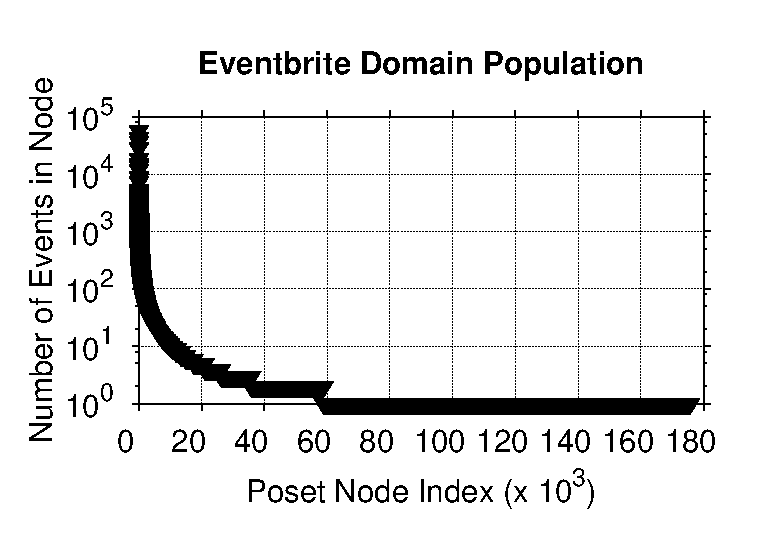
\includegraphics[clip,scale=0.5]{figs/eventbritepop.eps}
%	\vspace{-10pt}
%	\caption{The population of different nodes in the Eventbrite domain.}
%	\label{fig:eventbritepop}
%	\vspace{-10pt}
%	\end{center}
%\end{figure}
%\fi
%
%\ifpaper
%\begin{figure}[h]
%	\centering
%	\vspace{-10pt}
%	\subfigure{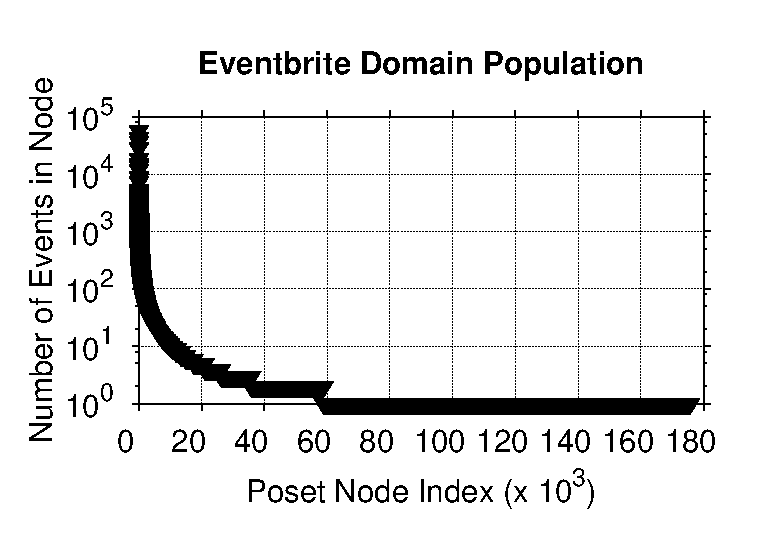
\includegraphics[clip,scale=0.32]{figs/eventbritepop.eps}\label{fig:eventbritepop}}
%	\hspace{-10pt}
%	\subfigure{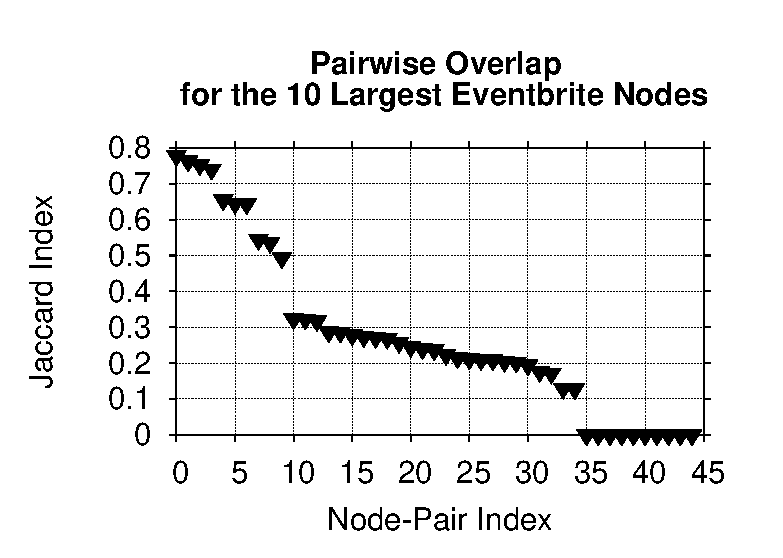
\includegraphics[clip,scale=0.32]{figs/overlaps.eps}\label{fig:eventbriteover}}
%	\vspace{-10pt}
%	\caption{(a) The population of different nodes and (b) pairwise overlaps for the 10 most populous nodes in the Eventbrite domain.}
%	\vspace{-10pt}
%\end{figure}
%\fi
%
%As mentioned before, a critical challenge in such large domains is deciding on the queries to ask. However, the hierarchical structure of the data domain presents us with an opportunity. One approach would be to perform a top-down traversal of the poset and issue queries at the different nodes. Nevertheless, this gives rise to a series of challenges: (i) how can one decide on the number of queries to be asked at each node, (ii) when should one progress to deeper levels of the poset and (iii) which subareas should be explored. We elaborate on these in \Cref{sec:prelims}. Next, we focus on the second challenge, i.e., the interdependencies across poset nodes. 
%\begin{example}
%We consider again the Eventbrite dataset and plot the pairwise overlaps of the ten most populous nodes in the domain. \Cref{fig:eventbriteover} shows the Jaccard index for the corresponding node pairs. As shown the event populations corresponding to these nodes overlap significantly. It is easy to see that when issuing queries at a certain domain node, we not only obtain events corresponding to this node but to other nodes in the domain as well.
%\end{example}
%A critical issue that stems from the overlaps across nodes is being able to decide how many answers to expect when issuing an additional query at a node whose underlying population overlaps with nodes associated with previous queries. In \Cref{sec:prelims}, we elaborate more on the dependencies across nodes of the poset.
%\iftr
%\begin{figure}
%	\begin{center}
%	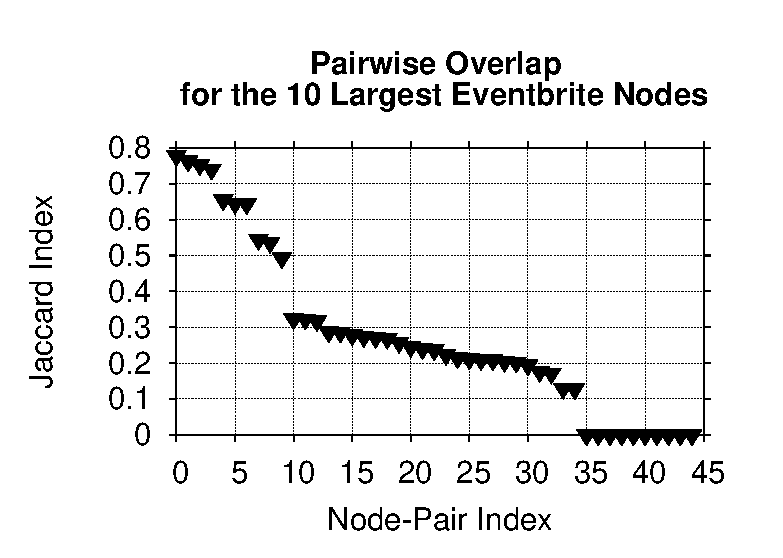
\includegraphics[clip,scale=0.5]{figs/overlaps.eps}
%	\vspace{-10pt}
%	\caption{Pairwise overlaps for the 10 most populous nodes.}
%	\label{fig:eventbriteover}
%	\vspace{-10pt}
%	\end{center}
%\end{figure}
%\fi
%\subsection{Contributions}
%\label{sec:contributions}
%Motivated by the examples above, we study the problem of crowdsourced entity extraction in the presence of long tail data. To effectively extract entities from the long tail we focus on {\em structured domains}. More precisely, we focus on domains described by a collection of attributes, each following a known {\em hierarchical structure}, i.e., we assume that for each attribute the corresponding hierarchy is known. Such hierarchies are usually dictated by the design of applications. \iftr Moreover, as controlling the overall extraction cost in large-scale applications is crucial we focus on {\em budgeted crowd entity extraction}. \fi
%
%We propose a novel algorithmic framework that exploits the structure of the domain to maximize the number of extracted entities under given budget constraints by targeting tail entities. In particular, we view the problem of entity extraction as a {\em multi-round adaptive optimization problem}. At  each round we exploit the information on extracted entities obtained by previous queries to adaptively select the crowd query that will maximize the {\em cost-gain} trade-off at each round. The gain of a query is defined as the {\em number of new unique entities extracted}. 
%
%We consider {\em generalized queries} that ask workers to provide us with entities from a domain $D$ and can also include an {\em exclude list}. In general such queries are of the type ``Give me $k$ more entities with attributes $\bar{X}$ that belong in domain $D$ and are not in $\{A, B, ...\}$''. Extending techniques from the species estimation and building upon the multi-armed bandits literature, we introduce a new methodology for estimating the gain for such generalized queries and show how the hierarchical structure of the domain can be exploited to increase the number of extracted entities. Our main contributions are as follows:
%
%\squishlist
%\item We formalize the notion of an exclude list for crowdsourced entity extraction queries and show how previously proposed gain estimators can be extended to handle such queries.
%\item We develop a new technique to estimate the gain of generalized entity extraction queries under the presence of little information, i.e., only when a small portion of the underlying entity population has been observed. We empirically demonstrate its effectiveness when extracting entities from sparse domains.
%\item We introduce an adaptive optimization algorithm that takes as input the gain estimates for different types of queries and identifies querying policies that maximize the total number of retrieved entities under given budget constraints. 
%\item Finally, we show that our techniques can effectively solve the problem of budgeted crowd entity extraction for large data domains on both real-world and synthetic data.
%\squishend

%
%
%
%\noindent\textbf{Our approach.} In this paper, we focus on entity extraction over {\em structured domains}, i.e., domains that can be fully described by a collection of attributes, each potentially exhibiting hierarchical structure, and demonstrate how exploiting the domain's structure can help us achieve the aforementioned goal. 
%In fact, most practical  applications that focus on aggregating and organizing information extracted from the crowd exhibit some form of structure. 
%
%
%To do so, we focus on entity extraction over {\em structured domains}, i.e., domains that can be fully described by a collection of attributes, each potentially exhibiting hierarchical structure, and demonstrate how exploiting the domain's structure can help us achieve the aforementioned goal. We point out that often the structure of domains in practical applications is already known by design. For example, Eventbrite categorizes extracted events based on a location taxonomy, an event type and their date. 
%
%Naturally, we should exploit the {\em structure} of the entity extraction domain, here, the entity-type and news portal, to minimize the number of duplicate extractions.
%
%\noindent\textbf{Structured entity domains.}
%An additional limitation of existing crowdsourced entity extraction techniques is that they are agnostic to the inherent {\em structure} that large-scale entity domains exhibit. In most practical scenarios, the entity domain can be described by a collection of attributes. For instance, if we consider the previous example of extracting modern philosophers, it is easy to see that the underlying domain can be described by attributes such as the nationality of a philosopher, her school of thought and her era. In fact many real-world crowdsourcing applications rely on s
%
%Exploiting the structure of the domain allows one to issue a collection of queries with different predicates corresponding to various attribute combinations. The latter is indeed used in real-world crowdsourcing applications. 
%
%
%\begin{example}
%We considered the application of enumerating ``people in the news''. We asked workers to consider five major online US news portals, ``New York Times'', ``Huffington Post'', ``Washington Post'', ``USA  Today'' and ``The Wall Street Journal'', and report five distinct people per HIT. We issued 600 HITs for \$0.20 per HIT served by 143 unique workers. To ensure the accuracy of our results we asked workers to provide us with a link corresponding to the extraction. These links were manually verified.  In total, we extracted 1,245 unique people. \Cref{fig:amtPop} shows the number of distinct workers that reported each person. As shown, there are 12 people that were reported by at least 20 different workers but there is a long tail of 842 people that were reported by one worker and 182 people reported by two workers. 
%\end{example}
%
%To understand the impact of duplicate extractions we conducted the following experiment. We asked workers via Amazon's Mechanical Turk (AMT)~\cite{mturk} to list 
%
%The situation only becomes worse when entities follow a skewed, long tail {\em popularity distribution}, i.e., a small number of entities have significantly higher probability of appearing in worker answers while a large number of {\em rare} entities have minuscule probability of being extracted. Next, we consider two crowdsourced entity extraction applications to demonstrate the presence of long tail popularity distributions and exemplify how they can lead to increased numbers of duplicate extractions.
%
%\textcolor{red}{
%\begin{enumerate}
%\item There are many extraction domains that exhibit structure. Different from simple domains such as list all ice cream flavors. Example, online aggregation of events, extraction of named entities etc. Diversification important. 
%\item Show why. Example, extract humans from different news papers. We see that we have different duplicate rates for different predicate combinations. How can we reason about which predicates to include in our queries? Work on example.
%\end{enumerate}
%}
%
%\begin{figure*}
%	\centering
%	\subfigure[Event popularity in EventBrite.]{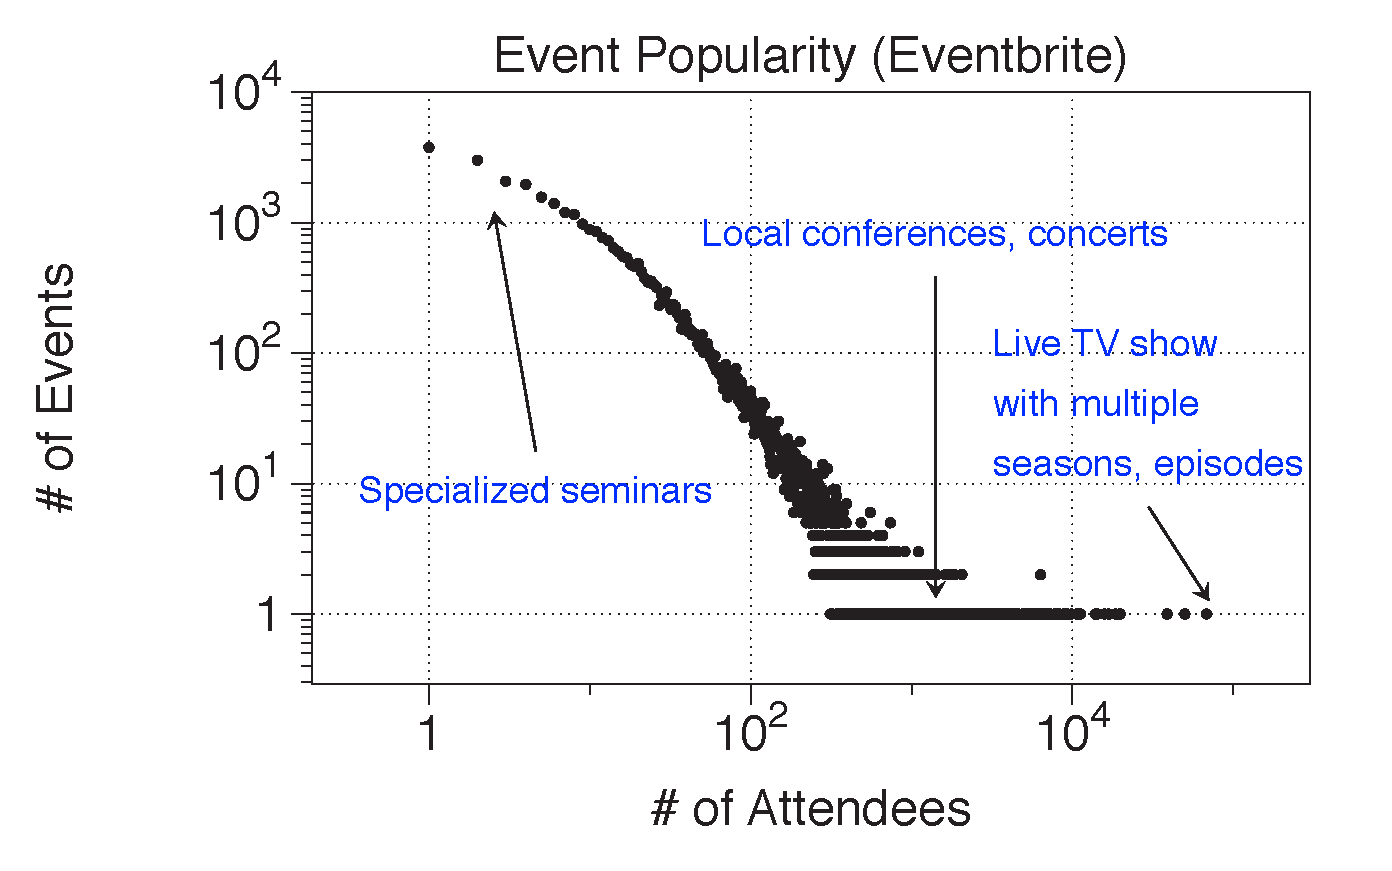
\includegraphics[clip,scale=0.35]{figs/eventPop.eps}\label{fig:eventPop}}
%	\subfigure[Entity popularity in crowdsourced people extraction.]{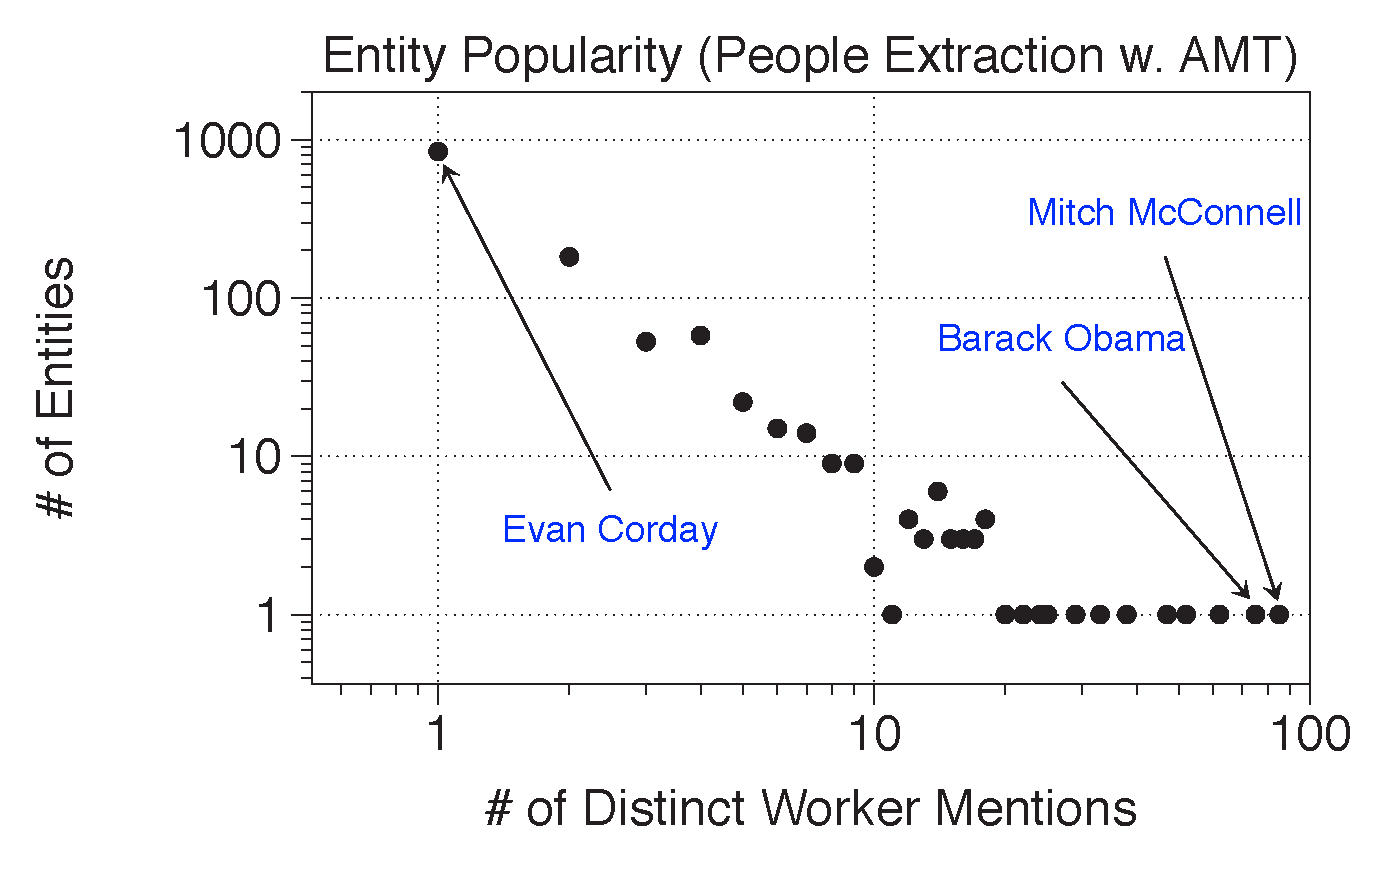
\includegraphics[clip,scale=0.35]{figs/amtPop.eps}\label{fig:amtPop}}
%	\caption{Entity popularity distributions exhibit long tails in real crowdsourced entity extraction applications.}
%\end{figure*}
%
%\begin{example}
%First, we consider Eventbrite~(\url{www.eventbrite.com}), an online event aggregator, that relies on crowdsourcing to compile a directory of events with detailed information about the location, type, date and category of each event. We collected a dataset via Eventbrite's API with events of 19 different categories from 63 different countries over a time period of 31 days. To measure the popularity of each event we use as a surrogate the number of attendees that registered for a specific event via Eventbrite.  In \Cref{fig:eventPop} we plot the number of registered attendees for different events grouping together events that had the same number of attendees. As shown, there is a large number of events with less than 100 attendees corresponding mostly to specialized seminars, and a small number of extremely popular events corresponding to concerts or live TV shows. 
%\end{example}
%
%\agp{not super clear how you plotted this}
%
%As we did not have immediate access to crowd workers for the aforementioned application, we also conducted a real crowdsourcing experiment via Amazon's Mechanical Turk (AMT)~\cite{mturk} that allowed us to precisely measure the popularity of extracted entities. 
%
%\begin{example}
%We asked workers to extract ``people in the news''. In particular, we asked them to consider five major online US news portals, ``New York Times'', ``Huffington Post'', ``Washington Post'', ``USA  Today'' and ``The Wall Street Journal'', and report five distinct people per HIT. We issued 600 HITs for \$0.20 per HIT served by 143 unique workers. To ensure the accuracy of our results we asked workers to provide us with a link corresponding to the extraction. These links were manually verified.  In total, we extracted 1,245 unique people. \Cref{fig:amtPop} shows the number of distinct workers that reported each person. As shown, there are 12 people that were reported by at least 20 different workers but there is a long tail of 842 people that were reported by one worker and 182 people reported by two workers. 
%\end{example}
%
%\agp{The examples are nice. Note that it's not clear what reporting means or
%what the workers are asked ---
%we need to stick to one of query, question, extract, report, etc.}
%
%\agp{CRUX, if we're using the acronym, needs to be introduced in the intro,
%not just in abstract.}
%
%\agp{Not super clear what the two graphs show -- i guess it's just that 
%we have a skewed probability distribution?
%can we also make the claim that: 
%there are actually just N entities:
%would it be possible to extract all entities using N or close to N crowd extractions, as opposed to using KN extractions, which is
%what we would have if we used repeated simple queries}
%
%\agp{got until here. }